\documentclass[french, 11pt, a4paper]{article} %langue française, police 11pt, format A4
\usepackage[french]{babel} % français, notamment pour la date, les défs, les thm., etc.
\usepackage[T1]{fontenc}
\usepackage{geometry} % pour les marges
\usepackage{array} % pour écrire l'application \phi en conclusion
\usepackage{amstext} % pour /text dans le mode math
\usepackage{amsmath} % pour les grandes fractions
\frenchsetup{StandardLists=true} % pour 'itemize' : des bullets et des interlignes pour une meilleure clarté
\usepackage{enumitem} %idem
\usepackage{amssymb} % pour les divers symboles, notamment \mathbb{}
\usepackage{stmaryrd} % pour les intervalles entiers
\usepackage{verbatim} % pour le formattage "mono"-like. Utilisation : \verb+TexteAFormatter+
\usepackage{listings}
\usepackage{xcolor}
\usepackage{graphicx}
\usepackage{makecell} % pour plusieurs lignes dans les cellules d'un tableau
\geometry{hmargin=1.3cm,vmargin=2cm} % marges élargies

%%% nouvelles commandes pour alléger l'écriture %%%

%% en mode math !! (entre des '$ $')
\newcommand{\Sc}{\mathcal{S}} % '\F' pour un F cursif
\newcommand{\N}{\mathbb{N}}
\newcommand{\R}{\mathbb{R}^*_+}

%% en mode text
\newcommand{\smb}{\smallbreak}


%% en-têtes
\title{Projet : Un problème de tournée de drones dans un contexte de déconfinement}
% corriger saut de ligne pour les auteurs
\author{PREKA Bruno, ZELLE Lars Yannick (681C)}
%% \date{\today}

%% début
\begin{document}


\maketitle



\section{Introduction}

Dans le contexte sanitaire actuel, un scénario fictif suggère l'isolement \emph{total} des personnes
atteintes de la Covid-19 dans leur domicile. Des drones sont alors réquisitionnés pour livrer des courses
à domicile.
\smb Dans chaque zone géographique, un unique dépôt (qu'on notera $1$ par la suite) stocke des ressources alimentaires et médicamenteuses.
Plusieurs contraintes se dessinent dans ce problème appartenant à la classe des problèmes de tournées de véhicules.
La contrainte garantissant que chaque client est visité une seule fois, ainsi que celle de la charge supportée par un drone,
y interviennent.
Le but du problème est de minimiser la distance parcourue par l'ensemble des drones.
\smb On résout ce problème à travers deux méthodes possibles :
\vspace{-0.2cm}
\begin{enumerate}
    \item Dite \emph{exacte}, elle assimile le problème en un problème d'optimisation
combinatoire, mais qui peut demander un temps d'exécution très important aux yeux des décideurs ;
    \item \emph{Approchée}, elle est une variante de la méthode de Clark et Wright.
\end{enumerate}

\subsection{Structures de données générales}

\subsubsection{Données du problème}
A partir de la fonction \verb+lecture_donnees+, on traduit les instances numériques fournies
par la structure de données 
\verb+donnees+ dont les champs sont dédiés au nombre de clients \verb+nbClients+ (y compris le dépôt), à
la \verb+capacité+ du drone, à la \verb+demande+ des clients et au distancier \verb+distance+. On retrouvera régulièrement les types suivants :
\begin{itemize}
    \item \verb+nbClients+ et \verb+capacite+ sont des entiers (on utilisera le type \verb+Int64+)
    \item \verb+demande+ est un vecteur d'entiers \verb+Vector{Int64}+ : la demande du client $i$ est renseigné dans ce vecteur, ce qui facilitera son accès.
    \item \verb+distance+ est une matrice à coefficients entiers \verb+Matrix{Int64}+. Ce type est équivalent à \verb+Array{Int64,2}+, ce qui sera utile pour manipuler des sous-matrices (restrictions de matrice).
\end{itemize}

\subsubsection{Ensemble des regroupements possibles : \texttt{S} ou $\Sc$}
On rappelle que l'ensemble des regroupements possibles est défini par :
\[\Sc := \Bigg\{ S \subseteq \llbracket 2,n \rrbracket : \sum_{j \in S} d_j \leq capacite \Bigg\} \]
Il est clair que la manipulation d'ensembles (type \verb+Set+) est simple, mais elle demande des temps d'exécution plus importants.
Il est donc plus que nécessaire de recourir à un "vecteur de vecteurs" au lieu d'un "ensemble d'ensembles", d'où
le type \verb+Vector{Vector{Int64}}+ pour l'ensemble des regroupements.

\subsubsection{Ensemble d'ensembles d'indices de tournées visitant le $i$-ème client : \texttt{AllS\_i} ou $\{S_i \subseteq \llbracket 1, |\Sc| \rrbracket\}$ }
La contrainte garantissant que chaque client soit visité une seule fois est donnée par :
\[ \sum_{j \in S_i} x_j = 1, i \in \llbracket 2,n \rrbracket, \]
où $S_i \subseteq \llbracket 1, |\Sc| \rrbracket$ est le sous-ensemble d'indices des tournées
contenant le client $i$.
Pour les mêmes raisons que ce qui précède, on opte pour un vecteur de vecteurs d'entiers, au lieu d'un ensemble d'ensembles d'entiers,
d'où le type \verb+Vector{Vector{Int64}}+.
\smb Pour un client $i$, l'accès à l'ensemble des indices des tournées le desservant se fait par \texttt{AllS\_i[i]} $=S_i$.

\subsubsection{Association tournée-distance minimale : \\ \texttt{l} 
$= \{(tournee_j,l_j) \: : \: \forall j \in \llbracket 1,|\Sc| \hspace{-0.15cm} \rrbracket,  \:
tournee_j \in \Sc 
\: \land \:
l_j = \min_{\text{\normalfont{TSP}}} \text{\normalfont{dist}}(tournee_j) \}$}

La fonction objectif (à minimiser) s'écrit :
\[ z = \sum_{j=1}^{|\Sc|} l_j x_j,\]
où $l_j$ désigne la distance minimale du regroupement $j \in \llbracket 1,|\Sc| \rrbracket$, calculée par la
fonction \verb+solveTSPExact+ de résolution du problème de voyageur de commerce (dit TSP).
Ainsi, une telle expression requiert de lier cette distance à son regroupement via un accès immédiat.
C'est pourquoi, le vecteur \verb+l+, constitué de couples $(tourn \text{é} e,distance_{\text{min}})$, intervient.
Il est de type \verb+Vector{Tuple{Vector{Int64},Int64}}+.
\smb Enfin, en termes d'accès, on a : $\forall j \in \llbracket 1,|\Sc| \rrbracket, \: l_j = $ \texttt{l[j][2]}.


\section{Résolution exacte}
\subsection{Fonction d'énumération des regroupements possibles des clients}
On appelle cette fonction \texttt{getSubsets\_recursive(P,S,capacite,demande,index,d,distances)},
où : \begin{itemize}
    \item \verb+P+ et \verb+toadd+ sont les vecteurs des indices à ajouter pour compléter un regroupement, \verb+toadd+ étant une copie de \verb+P+ ;
    \item \verb+S+ est l'ensemble des regroupements ;
    \item \verb+capacite+ désigne la capacité du drone ;
    \item \verb+demande+ est le vecteur de la demande des clients ;
    \item \verb+index+ est un curseur ;
    \item \verb+d+ est l'accumulateur courant de la demande pour respecter la condition de $\Sc$ ;
    \item \verb+distances+ est le distancier.
\end{itemize}

Derrière cette fonction, l'algorithme consiste à itérer (via \verb+index+) sur toutes les demandes des clients
et vérifier si la demande du client $i \in \llbracket 2,n \rrbracket$, accumulée à \verb+d+, est conforme à la capacité. Ainsi,
pour le client $i$ : 
\begin{enumerate}
    \item Si les demandes sommées sont en-dessous du seuil, on sauvegarde l'ensemble \verb+P+ des clients à ajouter dans \verb+toadd+
    et on ajoute le client suivant $i+1$ (à ajouter) à \verb+toadd+. Sinon, rien n'est fait et on passe à l'étape 4.
    \item On construit l'ensemble \verb+S+ $= \Sc$ en concaténant/réunissant \verb+S+ et \verb+[toadd]+.
    \item On répète le processus sur \verb+S+ et le client suivant $i+1$ et on compare le nouvel ensemble \verb+Snew+
    de regroupements : si \verb+Snew+ accueille de nouveaux regroupements, alors on les ajoute à \verb+S+.
    \item Une fois ce processus récursif terminé sur ce sous-groupe de clients $\{i,i+1,...,n\}$, on recommence pour le sous-groupe
$\{i+1,...,n\}$.
\end{enumerate}
\smb Par conséquent, il en résulte l'ensemble des regroupements attendu, à savoir $\Sc = $ \verb+S+.
\smb La fonction \texttt{getSubsets(capacite,demande,distances)} vient encapsuler la fonction récursive par l'appel
\texttt{getSubsets\_recursive([],[],capacite,demande,1,0,distances)}, avec \verb+index+ $=1$ et la distance \verb+d+ initialisée à $0$.

\subsection{Fonction déterminant la tournée et sa distance minimale dans un regroupement \texttt{Si}}
On appelle cette fonction \texttt{determineShortestCycle(Si,d)}, où : 
\begin{itemize}
    \item \verb+Si+ est un regroupement de clients à visiter (de type \verb+Vector{Int64}+) ;
    \item \verb+d+ est le distancier (\verb+Matrix{Int64}+).
\end{itemize}
\smb Puisque \verb+Si+ $\subseteq \llbracket 2,n \rrbracket$, il n'inclut pas le dépôt $1$. Ainsi, la réunion avec $\{1\}$
est primordiale pour passer par la fonction \verb+solveTSPExact(d)+ de résolution du TSP.
\smb De plus, il faut restreindre \verb+d+ au regroupement donné, d'où une sous-matrice
\verb+newd = d[Si,Si]+. Une telle opération est permise par l'équivalence entre les types
\verb+Matrix{.}+ et \verb+Array{.,2}+, comme évoqué précédemment.
\smb \verb+solveTSPExact+ retourne alors un couple $(tourn\text{é}e,dist_{\text{min}})$. Néanmoins, elle ne raisonne pas sur l'ensemble d'indices \verb+Si+, mais bien sur
$\llbracket 1,|\text{\texttt{Si}}| \rrbracket$. 
\smb Un réajustement des indices doit conserver la cohérence
des indices dans les tournées. Pour ce faire, on sait que le premier indice traité par \verb+solveTSPExact+ correspond au premier de \verb+Si+,
idem pour le deuxième, ainsi de suite... Puis, dans l'ordre, on a les correspondances suivantes :
\begin{itemize}
    \item le premier client $k_1$ de $tourn\text{é}e \longrightarrow$ client d'indice $k_1$ dans \verb+Si+ ;
    \item \dots
    \item le $i$-ème client $k_i$ de $tourn\text{é}e \longrightarrow$ client numéro \verb+Si[+$k_i$\verb+]+
    \item \dots
\end{itemize}


\section{Résolution approchée (brève)}

\section{Analyse des résultats issus des instances numériques ($A$ et $B$)}
\subsection{Résolution exacte}
A l'aide de la macro \texttt{@time} de Julia, on a mesuré les temps d'exécution (en secondes) des fonctions principales et les allocations mémoires.
Par ailleurs, on a également récupéré le nombre de regroupements pour chaque instance et les tailles minimale et maximale des regroupements.
Ces résultats sont donnés par les tableaux suivants :
\begin{center}
    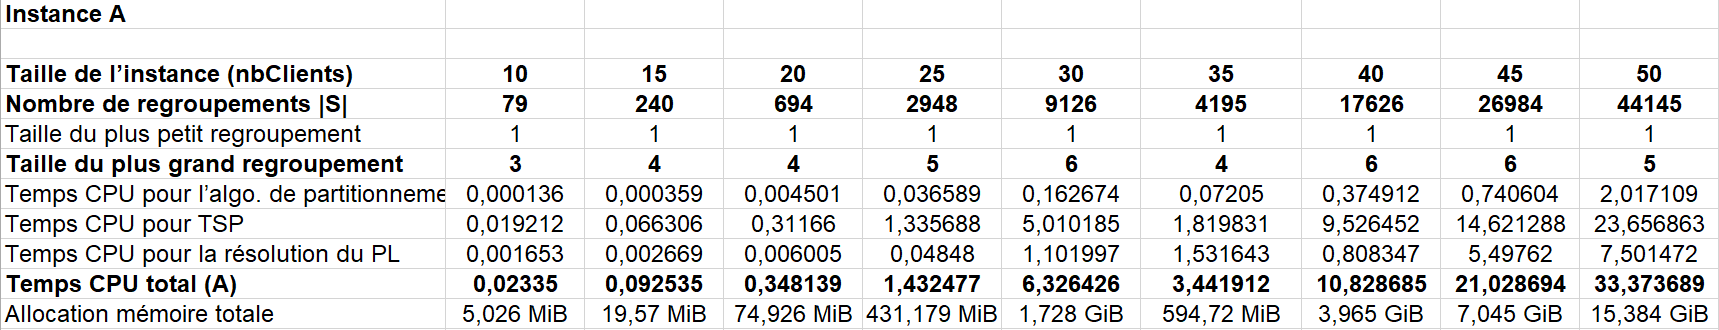
\includegraphics[scale=0.50]{ResExacte_InstA.PNG}
    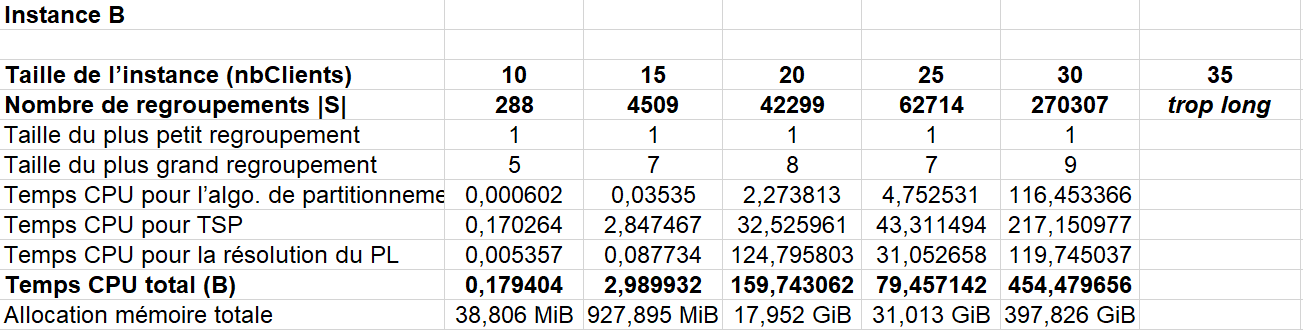
\includegraphics[scale=0.55]{ResExacte_InstB.PNG}
\end{center}



\end{document}
%% fin
